% ----------------------------------------------------------------------
%                   LATEX TEMPLATE FOR PhD THESIS
% ----------------------------------------------------------------------

% based on Harish Bhanderi's PhD/MPhil template, then Uni Cambridge
% http://www-h.eng.cam.ac.uk/help/tpl/textprocessing/ThesisStyle/
% corrected and extended in 2007 by Jakob Suckale, then MPI-CBG PhD programme
% and made available through OpenWetWare.org - the free biology wiki
% Modified to conform with University of Pennsylvania Thesis Requirements 
% by Alan Meert & David F. Moore, 2013, Dept. of Physics and Astronomy

%: Style file for Latex
%: Specify openright if printing double-sided, openany if single-sided
\documentclass[11pt, openany]{Latex/Classes/PhDthesisPSnPDF}
\usepackage{lipsum} % this just creates filler text when needed
\usepackage{UserDefs} %Define anything you might want to define in this file.

%: Macro file for Latex
% A macro that you may use frequently is the figuremacro 
\include{Latex/Macros/MacroFile1}

%
% WARNING!!!
%   Updating anything in this document other than the main document section is highly discouraged!
%


%: ----------------------------------------------------------------------
%:                  TITLE PAGE: name, degree,..\
% -----------------------------------------------------------------------

%if output to PDF then put the following in PDF header
\ifpdf  
    \pdfinfo { /Title  (\MyTitle)
               /Creator (TeX)
               /Producer (pdfTeX)
               /Author (\Me)
               /CreationDate (D:YYYYMMDDhhmmss)  %format D:YYYYMMDDhhmmss
               /ModDate (D:YYYYMMDDhhmmss)
               /Subject (Better Procrastination)
               /Keywords (Key to who?) }
    \pdfcatalog { /PageMode (/UseOutlines)
                  /OpenAction (fitbh)  }
\fi

\ifx\MySubTitle\undefined
    \title{\MakeUppercase{\MyTitle}}
\else
    \title{\MakeUppercase{\MyTitle}: \\ \small{\MySubTitle}}
\fi
% ----------------------------------------------------------------------
% Update UserDefs.sty instead of editing this part...
\ifpdf
  \author{\href{mailto:\MyEmail}{\Me}}
  \collegeordept{\href{http://www.physics.upenn.edu}{Physics and
Astronomy}}
  \university{\href{http://www.upenn.edu}{University of Pennsylvania}}

  % The crest is a graphics file of the logo of your research institution.
  % Place it in ./frontmatter/figures and specify the width
  \crest{
\includegraphics[scale=.5]{penn_fulllogo}}
  
% If you are not creating a PDF then use the following. The default is PDF.
\else
  \author{\Me}
  \collegeordept{Physics and Astronomy}
  \university{University of Pennsylvania}
  \crest{
\includegraphics[scale=.5]{penn_fulllogo}}
\fi

\degree{Doctor of Philosophy}
\degreedate{\MyEndDate}
\supervisor[\AdvisorTitle]{\MyAdvisor}
\gradchair[\GradChairTitle]{\GradChair}

\firstcomittee{\MyComOne}
\secondcomittee{\MyComTwo}
\thirdcomittee{\MyComThree}
\fourthcomittee{\MyComFour}
\fifthcomittee{\MyComFive}

\CopyrightStatement{This work is licensed under the Creative Commons
Attribution-NonCommercial-ShareAlike 3.0 License.\newline
\noindent To view a copy of this license, visit
\href{http://creativecommons.org/licenses/by‐ny‐sa/2.0/}{
http://creativecommons.org/licenses/by‐ny‐sa/2.0/}
}


%: --------------------------------------------------------------
%:                  FRONT MATTER: dedications, abstract,..
% --------------------------------------------------------------

\begin{document}

%\language{english}

% sets line spacing
\renewcommand\baselinestretch{1.2}
\baselineskip=18pt plus1pt

%: ----------------------- generate cover page ------------------------

\maketitle  % print the title page with above variables
\makecopyright % print the copyright page 

%: ----------------------- Other Frontmatter --------------------------
% Thesis Dedictation ---------------------------------------------------

\begin{dedication} %this creates the heading for the dedication page

\large\emph{To my bank account: Thanks for being underfed all these years. 
As a graduate student, I, too, know the feeling of hunger. Your willingness 
to support my poorly paid fantasy will soon pay off, and you will be slightly
more satisfied with my meager Postdoc salary.}

\end{dedication}

% ----------------------------------------------------------------------
% Thesis Acknowledgements ------------------------------------------------

\begin{acknowledgements}

Funding for this project was provided by the great spaghetti monster. The
great spaghetti monster proudly supports research through raining pasta 
on the hungry masses of graduate students. 

\end{acknowledgements}

% ------------------------------------------------------------------------




%: ----------------------- abstract ------------------------


% Thesis Abstract -----------------------------------------------------

\begin{abstracts}

Trust me \ldots I did stuff \ldots it was good. 350 words maximum here\ldots

\end{abstracts}

% ---------------------------------------------------------------------- 


%: ----------------------- contents ------------------------

\setcounter{secnumdepth}{3} % organisational level that receives a numbers
\setcounter{tocdepth}{3}    % print table of contents for level 3
\tableofcontents            % print the table of contents
% levels are: 0 - chapter, 1 - section, 2 - subsection, 3 - subsection


%: ----------------------- list of figures/tables ------------------------

\listoftables  % print list of tables
\listoffigures	% print list of figures

%: ----------------------- Preface ------------------------
% Thesis Preface -----------------------------------------------------

\begin{preface}

Perhaps you feel inclined to preface your work with poetic 
self-reflection about why you took up this project? Maybe a story 
that's kind of boring and ends with a joke that's not funny? Go for it!


\end{preface}

% ---------------------------------------------------------------------- 



%: --------------------------------------------------------------
%:                  MAIN DOCUMENT SECTION
% --------------------------------------------------------------

\mainmatter
%\renewcommand{\chaptername}{} % uncomment to print only "1" not "Chapter 1"


%: ----------------------- introduction file header -----------------------
\chapter{Introduction}

% the code below specifies where the figures are stored
\ifpdf
    \graphicspath{{introduction/figures/PNG/}{introduction/figures/PDF/}{introduction/figures/}}
\else
    \graphicspath{{introduction/figures/EPS/}{introduction/figures/}}
\fi

% ----------------------------------------------------------------------
%: ----------------------- introduction content ----------------------- 
% ----------------------------------------------------------------------

\section{put section name here} 
Any organised system requires energy, be it a machine of some kind or a live organism. Energy is needed to win the uphill battle against entropy and pull together lifeless molecules to be able to do something in this world, like complete a PhD\nomenclature[Zp]{Ph.D}{Acronym}.

\subsection{Name your subsection}
The machines that enable us to do science like sizzling electricity but at a controlled voltage\index{voltage}. Earth's living beings are no different, except that they have developed another preference. They thrive on various chemicals \citep{name06}. \lipsum


% ----------------------------------------------------------------------



	

\part{In the Beginning\ldots}

\chapter{Aims}

% the code below specifies where the figures are stored
\ifpdf
    \graphicspath{{example_chapter/figures/PNG/}{example_chapter/figures/PDF/}{example_chapter/figures/}}
\else
    \graphicspath{{example_chapter/figures/EPS/}{example_chapter/figures/}}
\fi


% ----------------------------------------------------------------------
%: ----------------------- content ----------------------- 
% ----------------------------------------------------------------------

\section{Junk}
This is where I put one of my very own defined functions!

\begin{table}
\centering
\begin{tabular}{|c|ccc|r|}
	\hline
$k$ &  $x_1^k$    &   $x_2^k$  & $x_3^k$   & remarks  \\
	\hline
0   & -0.3 & 0.6 & 0.7  &  \\
1   & 0.47102965 & 0.04883157 & -0.53345964  & *\\
2   & 0.49988691 & 0.00228830 & -0.52246185 & $s_3$ \\
3   & 0.49999976 & 0.00005380 & -0.52365600  & \\
4   & 0.5 & 0.00000307 & -0.52359743  & $\epsilon < 10^{-5}$ \\
7   & 0.5 & 0 & -0.52359878  & $\epsilon < \xi $ \\
	\hline
\end{tabular}
\caption[A table of important values]{This is a table with {\emph very} important values!!!!!}
\label{important_values}
\end{table}
    
\uv plane
    $$ \pdfdx{f}{x} $$

\section{Blah} 
\lipsum
\begin{figure}
\centering
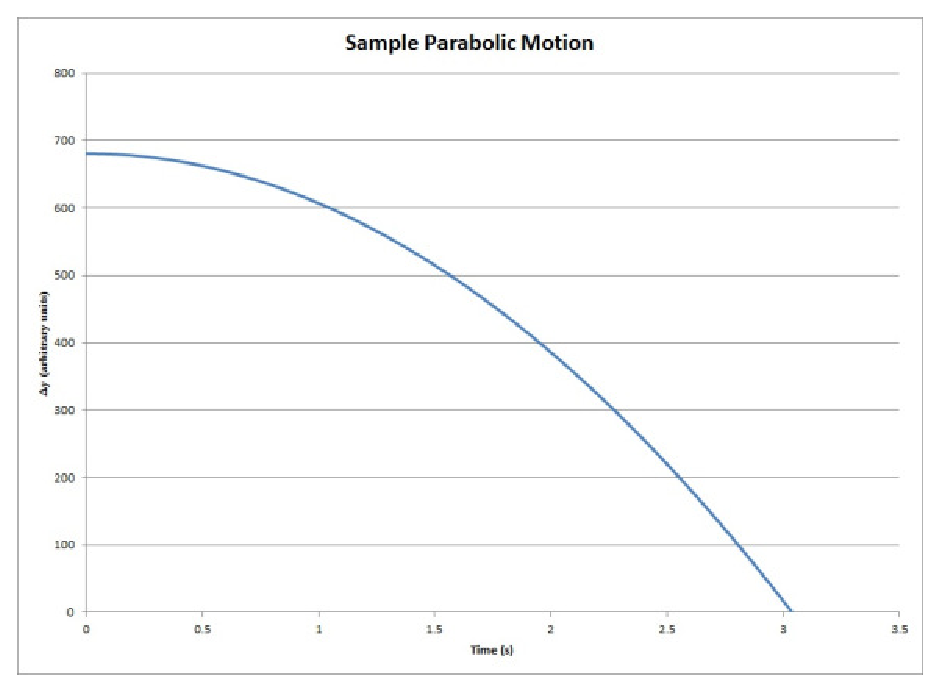
\includegraphics{parabolic_motion}
\caption[Parabolic Motion]{Here is parabolic motion as measured with science.}
\label{parabolic_motion}
\end{figure}
\lipsum
		
			
\part{A New Paradigm\ldots}

\begin{partChapter}
\chapter{Conclusion}

% the code below specifies where the figures are stored
\ifpdf
    \graphicspath{{colclusion/figures/PNG/}{colclusion/figures/PDF/}{colclusion/figures/}}
\else
    \graphicspath{{colclusion/figures/EPS/}{colclusion/figures/}}
\fi

% ----------------------------------------------------------------------
%: ----------------------- conclusion content ----------------------- 
% ----------------------------------------------------------------------

\section{Wrapping up\ldots}
I rest my case. \lipsum







\end{partChapter}
  


% --------------------------------------------------------------
%:                  BACK MATTER: appendices, refs,..
% --------------------------------------------------------------

%: ----------------------- Appendicies ------------------------
\begin{partChapter}

\begin{appendices}
\chapter{Some Appendix}
\lipsum
\section{first section}
\lipsum
\chapter{Another Appendix}
\lipsum
\end{appendices}

\end{partChapter}

% --------------------------------------------------------------
% Set backmatter mode after appendix so that chapter headings are
% not hidden
% --------------------------------------------------------------

\backmatter

%: ----------------------- glossary ------------------------

% Tie in external source file for definitions: /backmatter/glossary.tex
% Glossary entries can also be defined in the main text. See glossary.tex
% this file is called up by thesis.tex
% content in this file will be fed into the main document

% Glossary entries are defined with the command \nomenclature{1}{2}
% 1 = Entry name, e.g. abbreviation; 2 = Explanation
% You can place all explanations in this separate file or declare them in the middle of the text. Either way they will be collected in the glossary.

% required to print nomenclature name to page header
\markboth{\MakeUppercase{\nomname}}{\MakeUppercase{\nomname}}


% ----------------------- contents from here ------------------------

\nomenclature[Xe ]{11HUGS}{11 Mpc Halpha and Ultraviolet Galaxy Survey} 
\nomenclature[Zt ]{2MASS}{Two-Micron All Sky Sruvey}
\nomenclature[Am ]{M}{Mass of object}
\nomenclature[Gm ]{$\tau$}{Optical depth}
\nomenclature[Rs ]{$\ ^{*}$}{Conjugate}
\nomenclature[Ss ]{$\astrosun$}{relating to the sun (Sol)}
 

\clearpage
\begin{partChapter}
\begin{multicols}{2} % \begin{multicols}{#columns}[header text][space]
\begin{footnotesize} % scriptsize(7) < footnotesize(8) < small (9) < normal(10)

\printnomenclature[1.5cm] % [] = distance between entry and description
\label{nom} % target name for links to glossary

\end{footnotesize}
\end{multicols}
\end{partChapter}


%: ----------------------- bibliography ------------------------

% PhDbiblio-url2 = names small caps, title bold & hyperlinked, link to page 
\clearpage
\begin{partChapter}
\begin{multicols}{2} % \begin{multicols}{ # columns}[ header text][ space]
\begin{tiny} % tiny(5) < scriptsize(7) < footnotesize(8) < small (9)

\bibliographystyle{Latex/Classes/PhDbiblio-url2} % Title is link if provided
\renewcommand{\bibname}{References} % changes the header; default: Bibliography

\bibliography{./backmatter/references} % adjust this to fit your BibTex file

\end{tiny}
\end{multicols}
\end{partChapter}

% --------------------------------------------------------------
% Various bibliography styles exist. Replace above style as desired.

% in-text refs: (1) (1; 2)
% ref list: alphabetical; author(s) in small caps; initials last name; page(s)
%\bibliographystyle{Latex/Classes/PhDbiblio-case} % title forced lower case
%\bibliographystyle{Latex/Classes/PhDbiblio-bold} % title as in bibtex but bold
%\bibliographystyle{Latex/Classes/PhDbiblio-url} % bold + www link if provided

%\bibliographystyle{Latex/Classes/jmb} % calls style file jmb.bst
% in-text refs: author (year) without brackets
% ref list: alphabetical; author(s) in normal font; last name, initials; page(s)

%\bibliographystyle{plainnat} % calls style file plainnat.bst
% in-text refs: author (year) without brackets
% (this works with package natbib)
% --------------------------------------------------------------


%: ----------------------- Index ------------------------
\clearpage
\begin{partChapter}
\printindex
\end{partChapter}

\end{document}
